\documentclass[10pt,final,a4paper,oneside,onecolumn]{article}

%%==========================================================================
%% Packages
%%==========================================================================
\usepackage[a4paper,left=3.5cm,right=3.5cm,top=3cm,bottom=3cm]{geometry} %% change page layout; remove for IEEE paper format
\usepackage[T1]{fontenc}                        %% output font encoding for international characters (e.g., accented)
\usepackage[cmex10]{amsmath}                    %% math typesetting; consider using the [cmex10] option
\usepackage{amssymb}                            %% special (symbol) fonts for math typesetting
\usepackage{amsthm}                             %% theorem styles
\usepackage{dsfont}                             %% double stroke roman fonts: the real numbers R: $\mathds{R}$
\usepackage{mathrsfs}                           %% formal script fonts: the Laplace transform L: $\mathscr{L}$
\usepackage[pdftex]{graphicx}                   %% graphics control; use dvips for TeXify; use pdftex for PDFTeXify
\usepackage{array}                              %% array functionality (array, tabular)
\usepackage{upgreek}                            %% upright Greek letters; add the prefix 'up', e.g. \upphi
\usepackage[noadjust]{cite}                     %% citations; noadjust removes leading spaces
%\usepackage[round]{natbib}                     %% Author-year citations (remove package cite)
\usepackage{stfloats}                           %% improved handling of floats
\usepackage{multirow}                           %% cells spanning multiple rows in tables
%\usepackage{subfigure}                         %% subfigures and corresponding captions (for use with IEEEconf.cls)
\usepackage{subfig}                             %% subfigures (IEEEtran.cls: set caption=false)
\usepackage{fancyhdr}                           %% page headers and footers
\usepackage[official,left]{eurosym}             %% the euro symbol; command: \euro
\usepackage{appendix}                           %% appendix layout
\usepackage{xspace}                             %% add space after macro depending on context
\usepackage{verbatim}                           %% provides the comment environment
\usepackage[english]{babel}             %% language support
\usepackage{wrapfig}                            %% wrapping text around figures
\usepackage{longtable}                          %% tables spanning multiple pages
\usepackage{pgfplots}                           %% support for TikZ figures (Matlab)
\pgfplotsset{compat=1.14}
\usepackage[breaklinks=true,hidelinks,          %% implement hyperlinks (dvips yields minor problems with breaklinks;
bookmarksnumbered=true]{hyperref}   %% IEEEtran: set bookmarks=false)
%\usepackage[hyphenbreaks]{breakurl}            %% allow line breaks in URLs (don't use with PDFTeX)

\graphicspath{{figures/}}

%%==========================================================================
%% Define header/title stuff
%%==========================================================================
\newcommand{\progressreportnumber}{1}
\renewcommand{\author}{Erwin de Gelder}
\renewcommand{\date}{12 Oktober 2017}

%%==========================================================================
%% Fancy headers and footers
%%==========================================================================
\pagestyle{fancy}                                       %% set page style
\fancyhf{}                                              %% clear all header & footer fields
\fancyhead[L]{Summary of PhD Research topic. Start: October 1, 2017.}            %% define headers (LE: left field/even pages, etc.)
\fancyhead[R]{\author}                                  %% similar
\fancyfoot[C]{}                                         %% define footer

\begin{document}

\subsection*{Performance assessment methodology for automated vehicles using real-life driving data}

In recent years, much research has been conducted towards automated vehicles. It is generally accepted that testing of automated vehicles will become more and more important and complex. In order to investigate how an automated vehicle would perform in real-life traffic, real-life driving data can be used. This work focusses on developing a methodology for the assessment of automated vehicles using real-life driving data.

Figure \ref{fig:scheme} presents a schematic overview of the process of the assessment of an automated vehicle using real-life driving data. The starting point of the research is preprocessed data, i.e.\ the output of the second block in Figure \ref{fig:scheme}. The data preprocessing step includes the transformation of the sensor outputs into a reconstruction of the world, including the surrounding traffic objects. The primary goal of the research is to develop a methodology for the generation of the test cases using the preprocessed data, presented by the green blocks in Figure \ref{fig:scheme}. This will enable simulations, hardware-in-the-loop tests and real-life tests for assessing and evaluating automated vehicles. The simulation and evaluation (presented by the red blocks in Figure \ref{fig:scheme}) are not the focus of the research, as it is expected that these tasks are mostly performed by developers of automated vehicles (e.g.\ OEMs).

Five different topics will be addressed in the research:
\begin{enumerate}
	\item \emph{Event detection:}\,\,The first topic focusses on the detection of the events. The research, including the detection of events, requires an adequate definition of \emph{event}.
	\item \emph{Parametrization:}\,\,Parametrizing events is essential for enabling the generation of test cases. It needs to be investigated how the events can be parametrized such that the events can be reconstructed using the parameters while enabling the estimation of probability density functions that describe the underlying distribution of the parameters.
	\item \emph{Scenario mining:}\,\,The next topic involves defining and detecting scenarios. Scenarios are built using events. Furthermore, the scenarios describe the scenery, e.g., road layout and weather conditions. This topic addresses the ontology regarding a \emph{scenario} and the scenario mining.
	\item \emph{Test case generation:}\,\,The estimated probability density functions of the event parameters could be used for the generation of test cases. It is important that the generated test cases are realistic and that they resemble the variation found in real-life traffic.
	\item \emph{Completeness:}\,\,In order to draw conclusions on how the automated vehicle would perform in real-life traffic, it is necessary to know how representative the real-life driving dataset is. Therefore it is important to quantify how complete the dataset is. Is more data required? How much more data?
\end{enumerate}

In addition, several case studies, each involving one or more of these five topics, will be conducted.

\begin{figure}[h!]
	\centering
	\tikzstyle{block}=[node distance=5.2em, text width=4.5em, minimum height=7em, align=center, rounded corners=8pt, font=\small]
	\tikzstyle{my brace}=[decorate, decoration={brace, amplitude=10pt}]
	\tikzstyle{horz}=[node distance=2.7em]
	\tikzstyle{vert}=[node distance=4em]
	\begin{tikzpicture}[scale=0.95, every node/.style={transform shape}]
		% Draw the blocks
		\node[block, fill=blue!30](dc){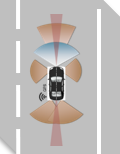
\includegraphics[width=3em]{data_collection.png} \\ Data collection};
		\node[block, fill=blue!30, right of=dc](dp){
\includegraphics[width=3em]{data_processing.png} \\ Data preprocessing};
		\node[block, fill=green!30, right of=dp](ed){
\includegraphics[width=4.2em]{event_detection.png} \\ Event detection};
		\node[block, fill=green!30, right of=ed](p){
\includegraphics[width=3em]{parametrisation.png} \\ Parame-trization};
		\node[block, fill=green!30, right of=p](s){
\includegraphics[width=3em]{scenarios.png} \\ Scenario mining};
		\node[block, fill=green!30, right of=s](tc){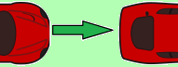
\includegraphics[width=4.2em]{test_cases.png} \\ Test case genera-tion};
		\node[block, fill=red!30, right of=tc](sim){
\includegraphics[width=4em]{simulation.png} \\ Simulation};
		\node[block, fill=red!30, right of=sim](eval){
\includegraphics[width=3em]{evaluation.png} \\ Evaluation};
		
		% Show completeness part
		\node[horz, left of=ed](b1){};
		\node[vert, below of=b1](b2){};
		\node[horz, right of=tc](b3){};
		\node[vert, below of=b3](b4){};
		\draw[my brace](b4) -- (b2) node[midway, yshift=-2em, align=center]{Completeness};
	\end{tikzpicture}
	\caption{Schematic overview of the process of the assessment of an automated vehicle using real-life data.}
	\label{fig:scheme}
\end{figure}

\end{document}